\section{qfileiconview.h File Reference}
\label{qfileiconview_8h}\index{qfileiconview.h@{qfileiconview.h}}


{\tt \#include $<$qiconset.h$>$}\par
{\tt \#include $<$qstring.h$>$}\par
{\tt \#include $<$qfileinfo.h$>$}\par
{\tt \#include $<$qdir.h$>$}\par
{\tt \#include $<$qtimer.h$>$}\par
{\tt \#include $<$qiconview.h$>$}\par
{\tt \#include $<$kurl.h$>$}\par
{\tt \#include \char`\"{}enum.h\char`\"{}}\par


Include dependency graph for qfileiconview.h:\begin{figure}[H]
\begin{center}
\leavevmode
\includegraphics[width=293pt]{qfileiconview_8h__incl}
\end{center}
\end{figure}


This graph shows which files directly or indirectly include this file:\begin{figure}[H]
\begin{center}
\leavevmode
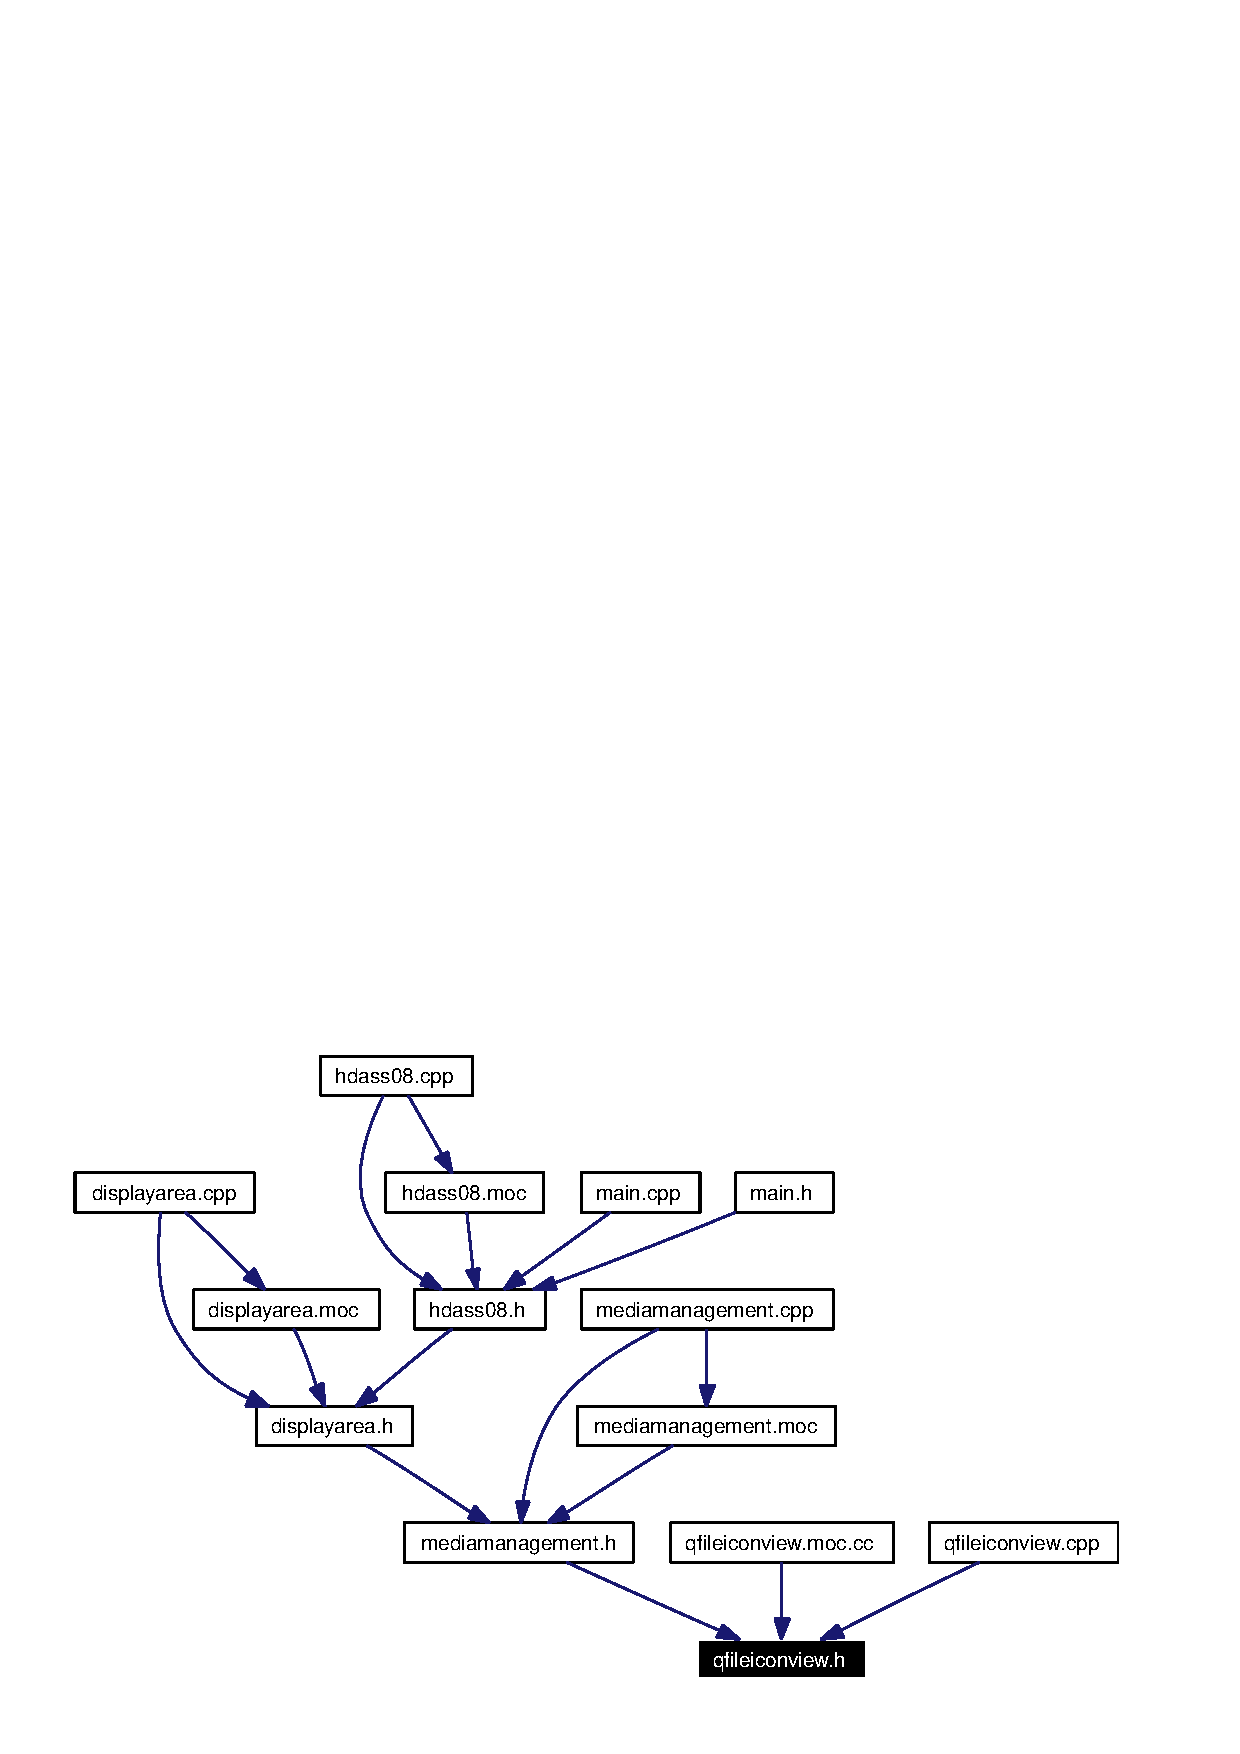
\includegraphics[width=268pt]{qfileiconview_8h__dep__incl}
\end{center}
\end{figure}
\subsection*{Classes}
\begin{CompactItemize}
\item 
class {\bf Qt\-File\-Icon\-Drag}
\item 
class {\bf Qt\-File\-Icon\-View}
\item 
class {\bf Qt\-File\-Icon\-View\-Item}
\end{CompactItemize}
\subsection*{Enumerations}
\begin{CompactItemize}
\item 
enum {\bf Floder\-Type} \{ {\bf Image} = 0, 
{\bf Music}
 \}
\end{CompactItemize}
\subsection*{Functions}
\begin{CompactItemize}
\item 
QPixmap $\ast$ {\bf add\-Border} (QPixmap $\ast$pix, bool has\-Alpha)
\end{CompactItemize}


\subsection{Enumeration Type Documentation}
\index{qfileiconview.h@{qfileiconview.h}!FloderType@{FloderType}}
\index{FloderType@{FloderType}!qfileiconview.h@{qfileiconview.h}}
\subsubsection{\setlength{\rightskip}{0pt plus 5cm}enum {\bf Floder\-Type}}\label{qfileiconview_8h_a3}


\begin{Desc}
\item[Enumeration values: ]\par
\begin{description}
\index{Image@{Image}!qfileiconview.h@{qfileiconview.h}}\index{qfileiconview.h@{qfileiconview.h}!Image@{Image}}\item[{\em 
Image\label{qfileiconview_8h_a3a0}
}]\index{Music@{Music}!qfileiconview.h@{qfileiconview.h}}\index{qfileiconview.h@{qfileiconview.h}!Music@{Music}}\item[{\em 
Music\label{qfileiconview_8h_a3a1}
}]\end{description}
\end{Desc}



Definition at line 56 of file qfileiconview.h.



\footnotesize\begin{verbatim}56                {
57 Image =0,
58 Music
59 };
\end{verbatim}\normalsize 


\subsection{Function Documentation}
\index{qfileiconview.h@{qfileiconview.h}!addBorder@{addBorder}}
\index{addBorder@{addBorder}!qfileiconview.h@{qfileiconview.h}}
\subsubsection{\setlength{\rightskip}{0pt plus 5cm}QPixmap$\ast$ add\-Border (QPixmap $\ast$ {\em pix}, bool {\em has\-Alpha})}\label{qfileiconview_8h_a2}




Definition at line 183 of file qfileiconview.cpp.

Referenced by Qt\-File\-Icon\-View\-Item::Qt\-File\-Icon\-View\-Item().



\footnotesize\begin{verbatim}184 {
185         //DAVID Read Background
186         QPixmap pbgxpm=QPixmap("/root/kde_application/hdass08/skin/bgxpm.png");
187         //DAVID Read Boarder Image
188         QImage ptop=QImage("/root/kde_application/hdass08/skin/border.png");
189         
190         //DAVID New a QPixmap res with size pix->size()
191         QPixmap res(pix->size());
192         
193         //Draw it on painter
194         QPainter p(&res);
195                 if(hasAlpha) 
196                         p.drawTiledPixmap (0, 0, pix->width(), pix->height(),pbgxpm);
197                 //DAVID draw broder to painter          
198                 p.drawImage(0, 0, ptop.scale(pix->width(), pix->height()));
199                 p.drawImage((int)floor((float)pix->width()/ptop.width()*14),
200                         (int)floor((float)pix->height()/ptop.height()*13),
201                         pix->convertToImage().smoothScale(
202                                 (int)ceil(pix->width()*0.79738562092),
203                                 (int)ceil(pix->height()*0.76691729323)));
204         p.end();
205         QImage a=res.convertToImage().scale(70,70);
206         QPixmap *temp=new QPixmap(a);
207         return temp;
208 }
\end{verbatim}\normalsize 
